\documentclass[UTF8]{ctexart}
    \usepackage{graphicx}
    \title{DgrAB Modeling}
    \author{Zhang Zhen}
\begin{document}
    \maketitle
    \section{Background Knowledge}
        \subsection{Part I}
            \textit{Ref: DgrA is a member of a new family of cyclic diguanosine monophosphate receptors and controls flagellar motor function in Caulobacter crescentus}

            DgrA is a PilZ homolog involved in mediating c-di-GMP-dependent control of C. crescentus cell motility.

            This protein family represents a class of specific diguanylate receptors and suggested a general mechanism for c-di-GMP binding and signal transduction. Increased concentrations of c-di-GMP or DgrA blocked motility in C. crescentus by interfering with motor function rather than flagellar assembly.

            The only flagellar protein whose concentration was severely affected in cells overexpressing dgrA was FliL which is required for flagellar rotation.

        \subsection{Part II}
            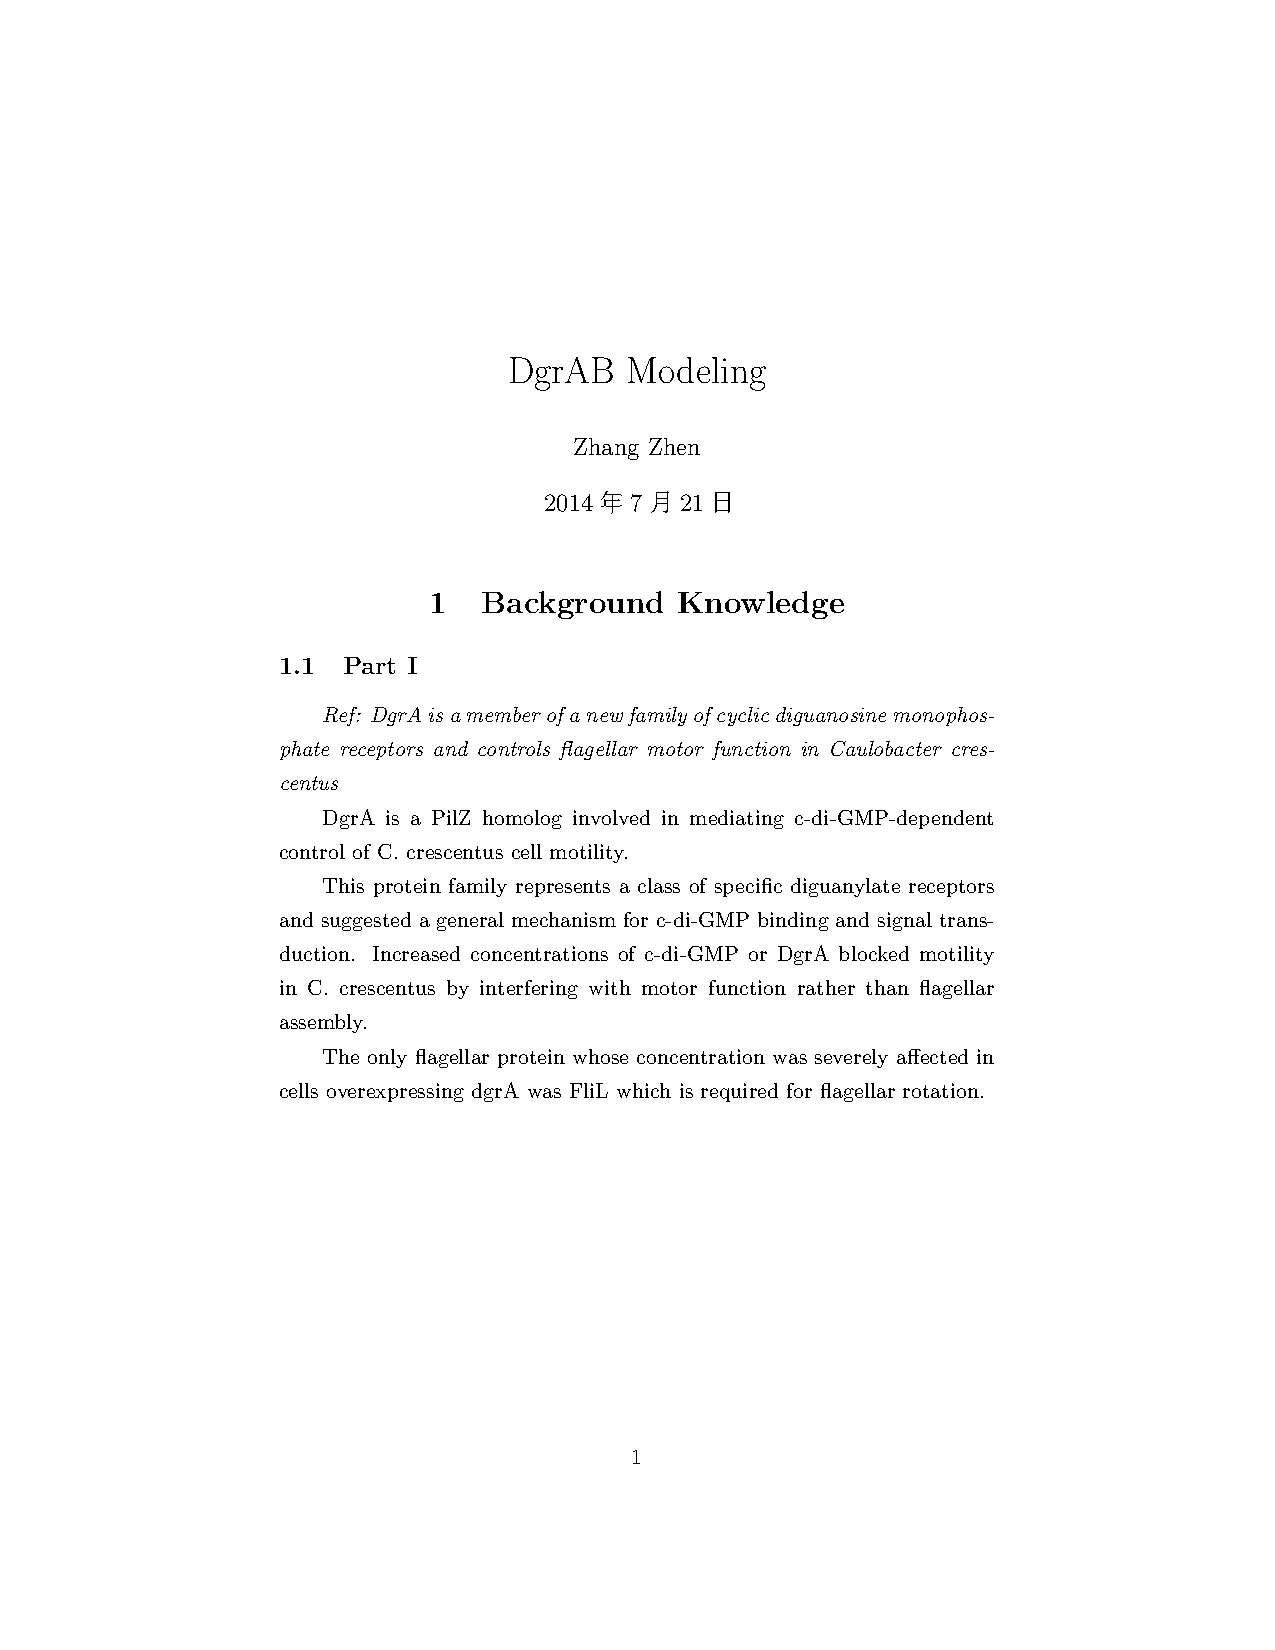
\includegraphics[width=3.00in]{DgrAB.png}\\
            \textit{Ref: Get the Message Out: Cyclic-Di-GMP Regulates Multiple Levels of Flagellum-Based Motility}\\\\
            \textbf{The explanation for this picture:}\\
            (Label 1) The DGC DgcA and an unidentified PDE set the steady-state levels of c-di-GMP, which (label 2) binds to DgrA and DgrB.\\
            (Label 3) Overexpression of DgrA decreases the steady-state levels of FliL.\\
            (Label 4) Since FliL mutants assemble paralyzed flagella, FliL may be integral to DgrA-dependent inhibition of rotation.\\
            (Label 5) Like DgrA, overexpression of DgrB inhibits flagellar rotation although it has no effect on FliL. The net effect of DgcA, DgrA, and DgrB is to impair rotation.\\

    \section{Modeling}
    \subsection{Abstract and ideas}
            The concentration of c-di-GMP is varying, and for our experiment we will promote its expression to inhibit rotation of flagella. It will bind to DgrA and DgrB. The resulting complex will have two routes to go: one is the [c-di-GMP\&DgrA] complex which will inhibit FliL, a protein bound to the membrane playing a key role in rotation of flagella. And the other route is that the DgrB will directly affect the rotation of flagella.

            It's clear that we know very poor about its real mechanism and there doesn't exist any quantitative analysis in the paper and research. All we have accomplished is to use control experiments to observe the basic relationships between these components.

            However, according to the paper, it has something to do with signal transduction and cell motor functionality where we can use our imagination to expand this topic. However, in this part, I will just show some basic block level modeling first
    \subsection{Definations:}
        \begin{enumerate}
        \item The concentration of c-di-GMP: $C_{X}$
        \item The total concentration of DgrA: $C_{A} = \alpha_{A}t - \beta_{A}C_{A}$
        \item The total concentration of DgrB: $C_{B} = \alpha_{B}t - \beta_{B}C_{B}$
        \item The maximum transcriptional rate of FliL: $\alpha_{F}$
        \item The actual transcriptional rate of FliL: $\alpha_{F}^{*}$
        \item The total concentration of FliL: $C_{F} = \alpha_{F}^{*}t - \beta_{F}C_{F}$
        \item The concentration of DgrA\&c-di-GMP complex: $C_{A}^{*}$
        \item The concentration of DgrB\&c-di-GMP complex: $C_{B}^{*}$
        \item The dissociation rate of DgrA\&c-di-GMP complex: $Kd_{AX}$
        \item The dissociation rate of DgrB\&c-di-GMP complex: $Kd_{BX}$
        \item The degradation rate of repressing effect: $k$
        \end{enumerate}
    \section{Equations:}
        \begin{enumerate}
        \item Binding of c-di-GMP with DgrA and DgrB: 
            $$C_{A}^{*} = C_{A} - C_{AX} = C_{A} - Kd_{AX}*C_{A}*C_{X}$$
            $$C_{B}^{*} = C_{B} - C_{BX} = C_{B} - Kd_{BX}*C_{B}*C_{X}$$
        \item The repressing effect of DgrA\&c-di-GMP complex: 
            $$\alpha^{*}_{F} = \frac{\alpha_{F}}{1+\frac{C_{A}^{*}}{k}}$$
        \item The rotation effect: 
            $$Rot = f(C_{F}, C_{B}^{*})$$
        \end{enumerate}

\end{document} 